\subsubsection{Sequence Diagram - Module Phân quyền}

Đảm bảo an toàn bảo mật và phân quyền chính xác là yêu cầu cốt lõi của hệ thống. Biểu đồ tuần tự tại Hình \ref{fig:seq_auth} mô tả chi tiết quy trình đăng nhập và cơ chế tự động tải quyền hạn (Permissions) kết hợp với chiến lược Caching để tối ưu hiệu năng.

\begin{figure}[H]
    \centering
    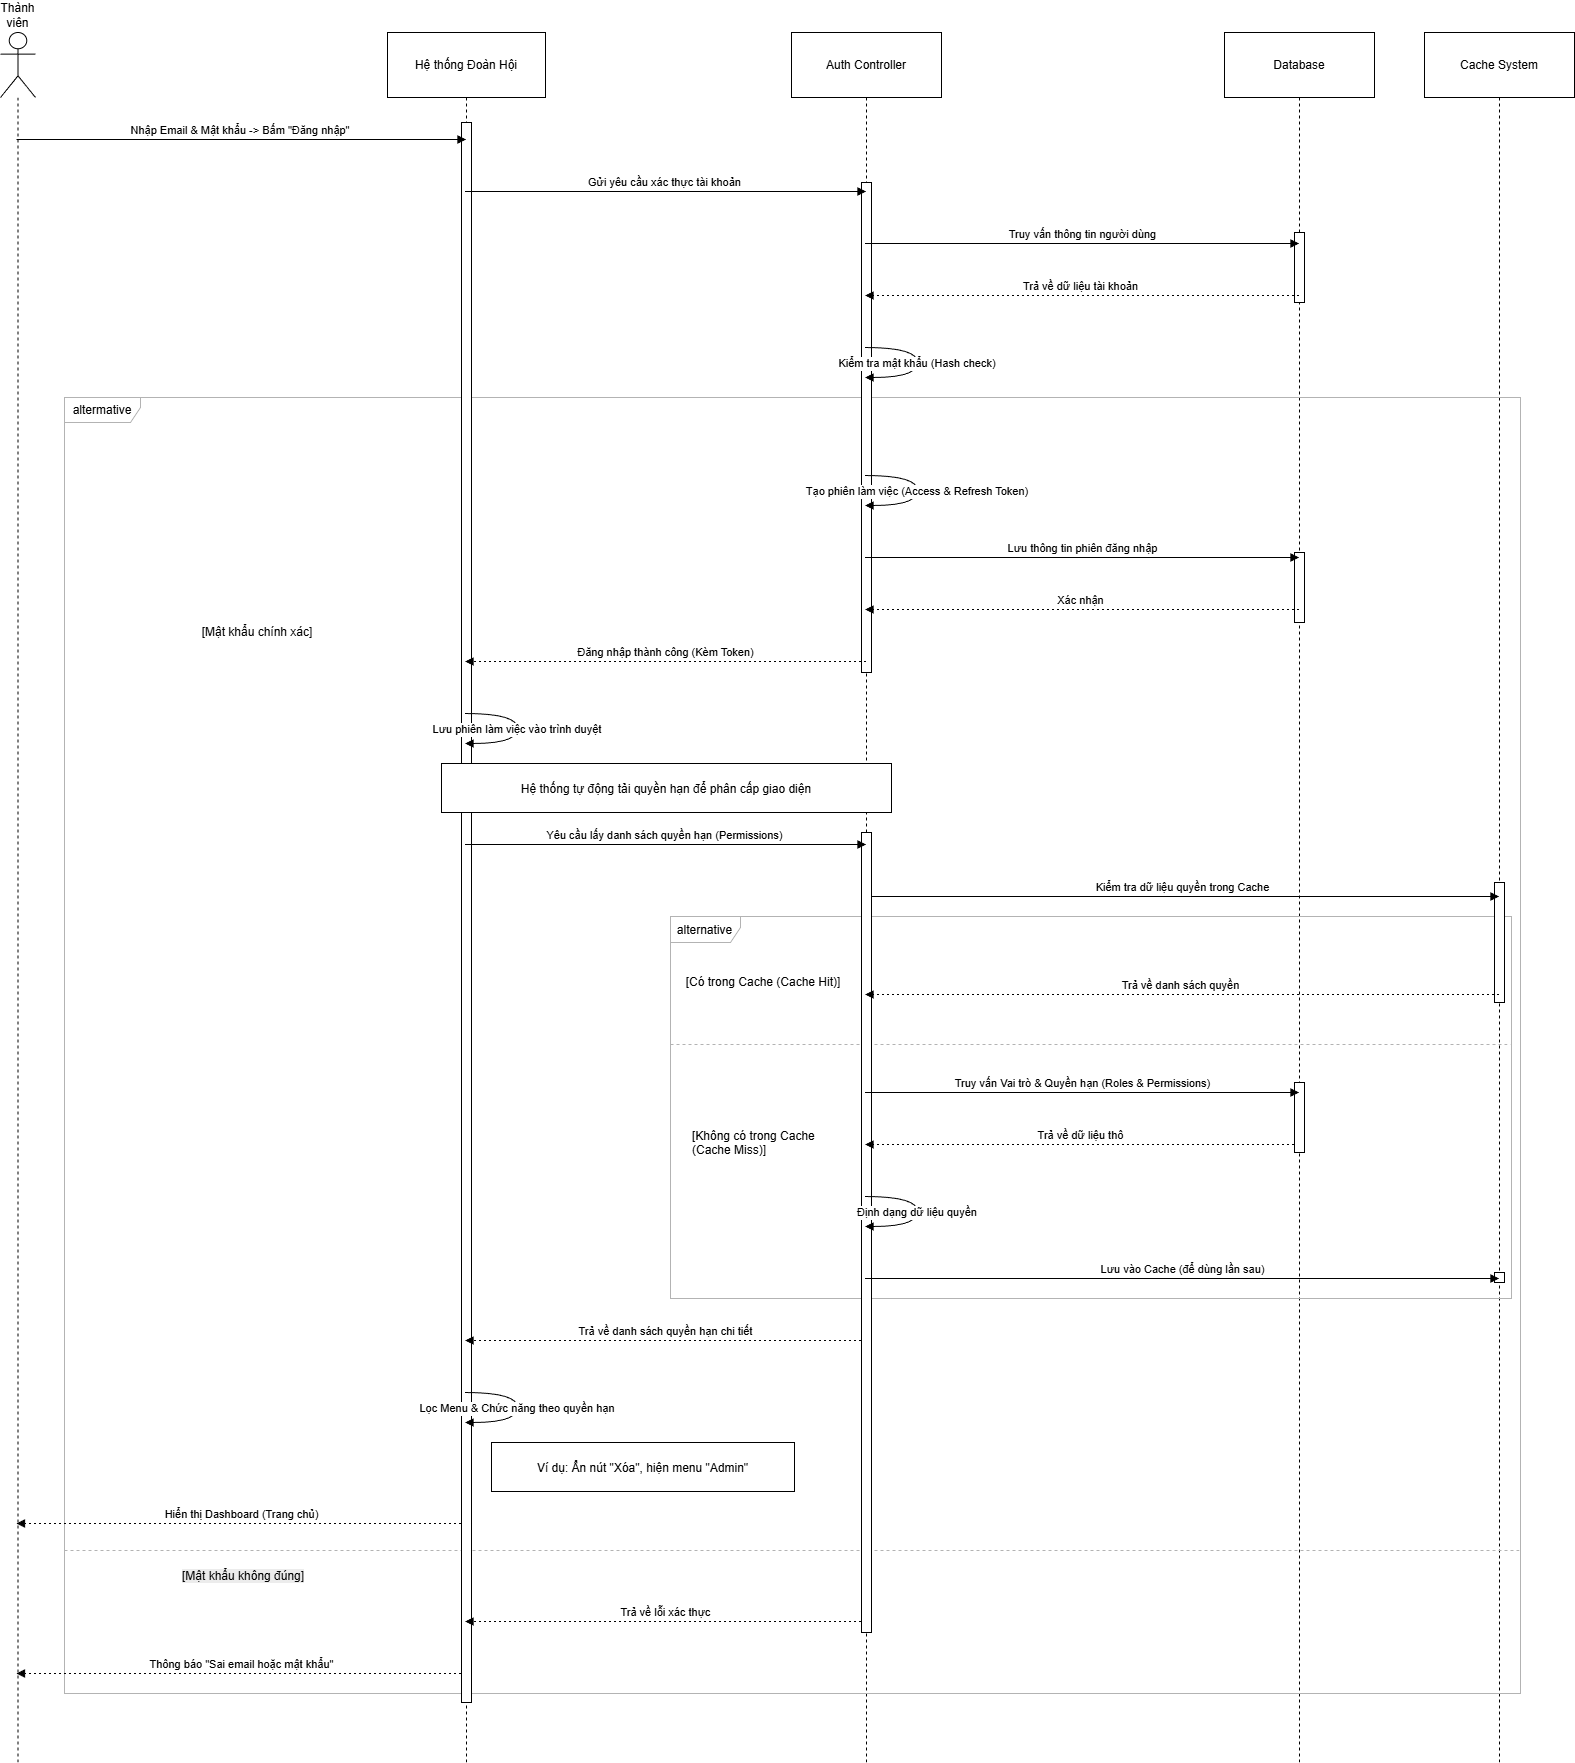
\includegraphics[width=1.0\textwidth]{Images/sequence-diagram/SQ05_authorization-sequence.drawio.png} 
    \caption{Sequence Diagram - Luồng hoạt động cơ chế phân quyền}
    \label{fig:seq_auth}
\end{figure}

Quy trình được chia thành ba giai đoạn xử lý chính:

\paragraph{Giai đoạn 1: Xác thực người dùng (Authentication)}
Khi thành viên nhập thông tin đăng nhập, hệ thống thực hiện các bước kiểm tra bảo mật nghiêm ngặt:
\begin{itemize}
    \item \textbf{Kiểm tra thông tin:} \textit{Auth Controller} truy vấn thông tin từ cơ sở dữ liệu và thực hiện so khớp mật khẩu đã được mã hóa (\textit{Password Hashing Check}).
    \item \textbf{Cấp phát phiên làm việc:} Nếu thông tin chính xác, hệ thống khởi tạo phiên làm việc bằng cách cấp phát cặp khóa \textit{Access Token} và \textit{Refresh Token}. Thông tin phiên này cũng được lưu vết vào cơ sở dữ liệu để quản lý bảo mật.
\end{itemize}

\paragraph{Giai đoạn 2: Tải quyền hạn và Tối ưu hóa với Cache}
Sau khi đăng nhập thành công, hệ thống tự động thực hiện quy trình phân quyền (Authorization) để xác định phạm vi truy cập của người dùng. Để giảm tải cho cơ sở dữ liệu khi lượng truy cập lớn, nhóm áp dụng chiến lược \textbf{Caching} (Lưu bộ nhớ đệm):
\begin{enumerate}
    \item Hệ thống kiểm tra danh sách quyền hạn của người dùng trong \textit{Cache System}.
    \item \textbf{Trường hợp Cache Hit:} Nếu dữ liệu quyền đã có sẵn trong bộ nhớ đệm, hệ thống trả về ngay lập tức, giúp giảm độ trễ phản hồi xuống mức thấp nhất.
    \item \textbf{Trường hợp Cache Miss:} Nếu chưa có trong Cache, hệ thống mới thực hiện truy vấn phức tạp (Join bảng Vai trò \& Quyền hạn) từ Database, sau đó định dạng dữ liệu và lưu ngược vào Cache cho các lần truy cập sau.
\end{enumerate}

\paragraph{Giai đoạn 3: Phân cấp giao diện (UI Adaptation)}
Dựa trên danh sách quyền hạn nhận được, \textit{Hệ thống Đoàn Hội} (Frontend) thực hiện lọc và hiển thị giao diện động:
\begin{itemize}
    \item Các chức năng không thuộc quyền hạn của người dùng (ví dụ: nút "Xóa", menu "Quản trị") sẽ bị ẩn đi.
    \item Người dùng được chuyển hướng đến Trang chủ (Dashboard) với giao diện được cá nhân hóa theo đúng vai trò.
\end{itemize}

Quy trình này đảm bảo tính toàn vẹn dữ liệu và ngăn chặn các truy cập trái phép vào các chức năng nhạy cảm của hệ thống.